%% results_07_shapiq_position.tex
%% Section 7 (or Appendix / Discussion): What the results mean for shapiq
%%
%% This file cross-references the findings from:
%%   results_05a_rq1.tex  (RQ1: Dimensionality Scaling)
%%   results_06_analysis.tex  (Cross-Cutting Analysis)
%% to characterise shapiq's position relative to the other libraries.
%%
%% All numbers come from results/converted/ (rq1_results_converter.py +
%% rq2_results_converter.py run on the RQ1+RQ2 benchmark CSVs).
%% ============================================================

\section{What the Results Mean for \shapiq}
\label{sec:shapiq-position}

The benchmark was designed to be library-agnostic, but \shapiq\ is the
primary library under development in this project.
This section synthesises the findings from
Sections~\ref{sec:us1} and~\ref{sec:analysis} into a direct assessment of
where \shapiq\ stands relative to its competitors, where it still lags,
and what the data implies for its development priorities.

% ─────────────────────────────────────────────────────────────────────────────
\subsection{Computational Speed: Behind SHAP, Ahead of the Pack at Scale}
\label{sec:shapiq-speed}

\paragraph{Absolute runtime.}
In the standard dimensionality benchmark (budget~512, pooled over four
models and ten seeds), \shapiq\ kernel is \textbf{5$\times$ slower than
SHAP kernel} at every tested feature count: 1.3\,s vs.\ 0.26\,s at 14
features, rising to 3.5\,s vs.\ 0.65\,s at 79 features.
This overhead is consistent across the entire 14--256 feature range
(ratio 4.1--5.3$\times$), indicating a fixed relative cost rather than a
scaling pathology.
The most likely source is \shapiq's interaction-aware coalition generation,
which evaluates a broader set of subset sizes than SHAP's permutation or
kernel variants.

\paragraph{Scaling with dimensionality.}
Despite the constant overhead, \shapiq\ kernel and permutation both scale
gracefully: at 256 features (budget~1\,024, time-capped LightSHAP runs
excluded) \shapiq\ kernel completes in 5.2\,s and \shapiq\ permutation in
7.5\,s, second only to SHAP kernel (3.6\,s) and SHAP permutation
(6.3\,s).
Crucially, \shapiq\ \emph{never triggers the execution cap} across the
entire standard benchmark grid (Sections~\ref{sec:rq1-feasibility}), whereas
LightSHAP fails in 62--75\,\% of runs at 256 features.
This makes \shapiq\ the only library other than SHAP and DALEX that can be
reliably deployed at up to 256 features without timeout risk.

\paragraph{Budget scaling.}
For both \shapiq\ variants, the runtime ratio $t_{1024}/t_{512}$ is
\textbf{below 2} (kernel: median 1.25; permutation: median 1.56), meaning
that doubling the coalition budget costs less than twice the runtime.
This suggests a fixed per-run overhead (model loading, coalition set
construction) that does not scale with the number of samples.
In contrast, SHAP kernel and permutation sit much closer to the 2$\times$
line (see Figure~\ref{fig:rq1-budget} in Section~\ref{sec:us1}), indicating
that their runtimes are dominated by model evaluations rather than overhead.

\paragraph{Extreme dimensionality (1,000 features).}
In the separate stress test (Section~\ref{sec:rq1-stress}), all \shapiq\
configurations complete successfully at 1\,000 features in 21--41\,s
across all four model types, while LightSHAP requires up to 3.5\,h.
\shapiq\ is the \textbf{second-fastest feasible library} at this
dimensionality, behind SHAP kernel (13--18\,s) and ahead of SHAP
permutation (15--22\,s) and DALEX permutation (70--71\,s).

\finding{%
  \shapiq\ is 4--5$\times$ slower than SHAP kernel at all standard feature
  counts but never times out and scales reliably to 1\,000 features.
  Its sublinear budget overhead means that at very high budget levels the
  cost gap vs.\ SHAP narrows in practice.%
}

% ─────────────────────────────────────────────────────────────────────────────
\subsection{Accuracy: Strong Convergence Potential, Weak Starting Point}
\label{sec:shapiq-accuracy}

\paragraph{Error at low budget.}
\shapiq\ kernel has the \textbf{highest error at budget~128} of all tested
methods: a median relative MAE of 22.7\,\% against the
\texttt{shap\_true\_value} oracle.
\shapiq\ permutation is similarly high at 18.3\,\%.
Both are dominated on the runtime--accuracy Pareto frontier
(Section~\ref{sec:pareto}) by SHAP kernel and SHAP permutation, which
achieve lower error \emph{and} shorter runtimes at the same budget.
This weakness at low budget is a known consequence of the interaction-aware
coalition weighting: \shapiq\ samples a richer set of coalitions but needs
more samples before the estimates stabilise.

\paragraph{Convergence rate.}
\shapiq\ kernel shows the \textbf{fastest convergence rate of any tested
method}: a 7.6$\times$ error reduction from budget~128 (22.7\,\%) to
budget~2\,048 (3.0\,\%), beating all competitors
(Table~\ref{tab:convergence} in Section~\ref{sec:analysis}).
At budget~2\,048, \shapiq\ kernel reaches a median relative MAE of 3.0\,\%
and a Spearman rank correlation of 0.991 with the exact oracle---comparable
to SHAP kernel (3.0\,\%, $\rho = 0.994$) and DALEX permutation (5.0\,\%,
$\rho = 0.991$) at the same budget.
\shapiq\ permutation converges more slowly (4.3\,\% at budget~2\,048,
$\rho = 0.992$) and remains slower in runtime (38.4\,s vs.\
2.2\,s for \shapiq\ kernel).

\paragraph{Pareto position.}
Despite the strong convergence, \shapiq\ kernel at budget~2\,048 is still
dominated by two configurations: LightSHAP permutation at budget~128
(lower error and shorter runtime) and SHAP permutation at budget~2\,048
(slightly lower error at similar runtime).
\shapiq\ permutation at all budgets is dominated by a large number of
competing configurations and is not on the efficient frontier under any
combination of runtime and MAE considered here.

Figure~\ref{fig:shapiq-convergence} illustrates these trajectories.

\begin{figure}[ht]
  \centering
  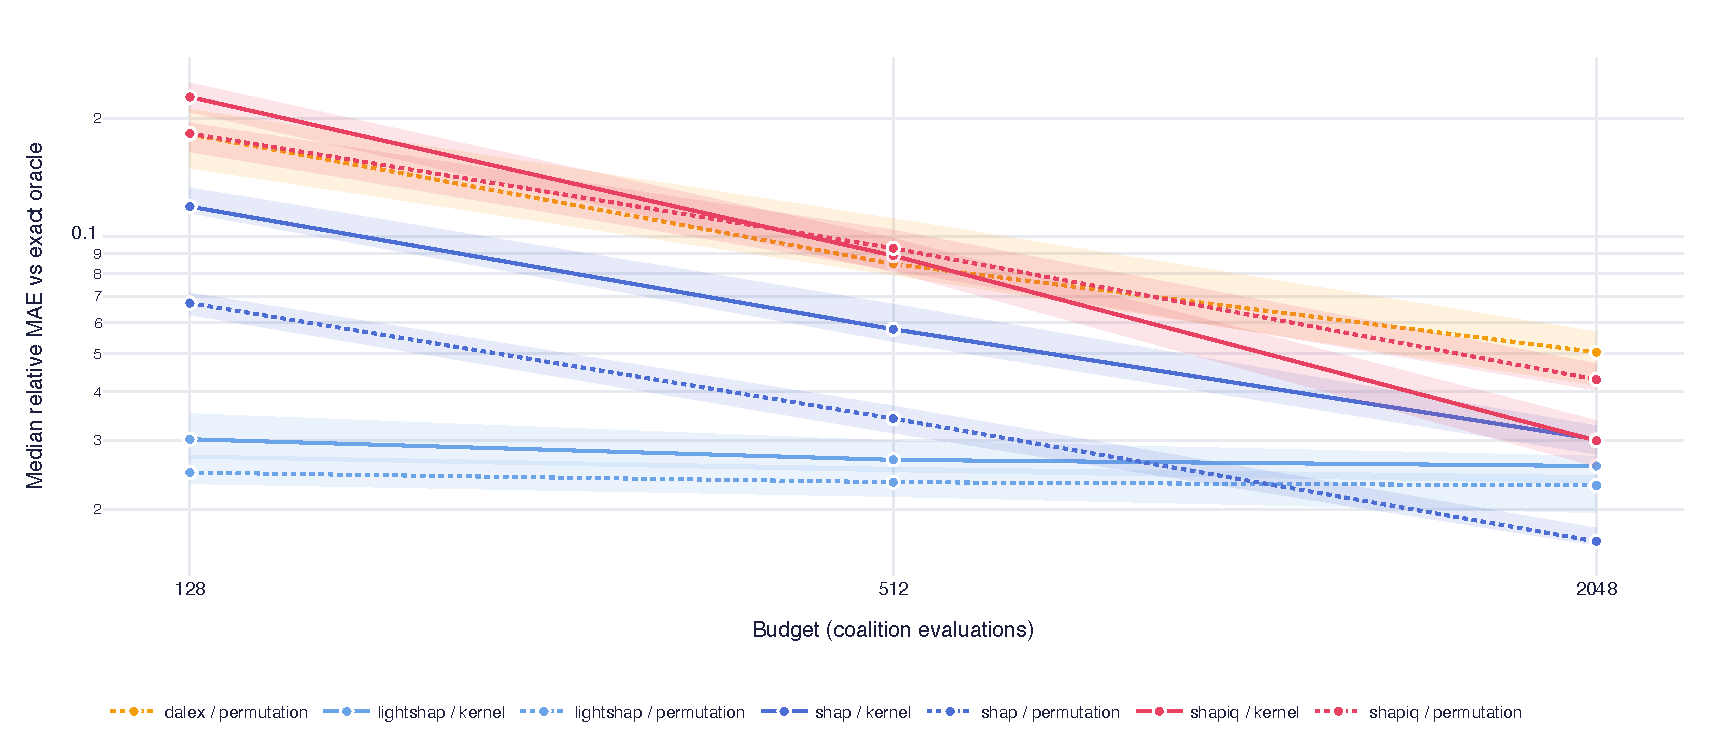
\includegraphics[width=\linewidth]{figures/rq2_f1_convergence}
  \caption{%
    Error convergence over budget for all seven method configurations
    (reproduced from Figure~\ref{fig:rq2-convergence} for reference).
    \shapiq\ kernel (dark blue, solid) starts with the highest error at
    budget~128 but achieves the steepest convergence slope, reaching parity
    with SHAP kernel by budget~2\,048.
    \shapiq\ permutation (dark blue, dashed) converges more slowly and
    remains above \shapiq\ kernel throughout.
  }
  \label{fig:shapiq-convergence}
\end{figure}

\paragraph{Sign agreement and stability.}
\shapiq\ kernel has the \textbf{lowest sign agreement of all methods at
every budget} (0.87 at budget~128, 0.92 at budget~512, 0.96 at
budget~2\,048), meaning it most frequently assigns the wrong direction
(positive vs.\ negative) to attributions at low-to-medium budgets.
Sign agreement does not reach 0.99 even at budget~2\,048, unlike
LightSHAP permutation (0.99 already at budget~128) and most other methods.
For applications where the sign of an attribution is the critical
decision criterion---e.g.\ identifying whether a feature increases or
decreases a prediction---\shapiq\ kernel requires at least budget~2\,048
and even then sits at the lower end of the tested methods.

\shapiq\ kernel also has the \textbf{widest seed-to-seed variability} at
budget~512: the interquartile range of relative MAE divided by the median
is 2.31, compared to 0.75 for LightSHAP kernel and 1.51 for
\shapiq\ permutation.
This means that a single run of \shapiq\ kernel at budget~512 may be
substantially worse than the median; practitioners who need reproducible
estimates should use budget~2\,048 or ensemble multiple seeds.

\finding{%
  \shapiq\ has the worst accuracy at budget~128 but the fastest
  convergence rate (7.6$\times$ error reduction to budget~2\,048), at
  which point it reaches parity with SHAP kernel.
  Sign agreement and seed stability are the weakest of all tested methods
  at low-to-medium budgets; a budget of at least 2\,048 is needed for
  reliable directional attributions.%
}

% ─────────────────────────────────────────────────────────────────────────────
\subsection{What Makes \shapiq\ Distinct}
\label{sec:shapiq-distinction}

The benchmark measures \emph{Shapley value approximation quality and speed}
on the same footing for all libraries.
From that perspective, \shapiq\ is currently outperformed by SHAP kernel
on the runtime--accuracy Pareto frontier at all budgets, and by LightSHAP
on accuracy at low and medium budgets.

However, the benchmark does not capture the feature that differentiates
\shapiq\ architecturally: its native support for \textbf{Shapley
interaction indices (SII)}, which assign attribution credit to pairs and
higher-order subsets of features rather than individual features.
None of the other benchmarked libraries support this directly.
The following points contextualise the benchmark results in light of this
distinction.

\begin{itemize}

  \item \textbf{The convergence advantage is structurally meaningful.}
  \shapiq's interaction-aware coalition weighting is designed to reduce
  the variance of the Shapley value estimator when interactions are
  present~\cite{shapiq2024}.
  The 7.6$\times$ MAE reduction from budget~128 to~2\,048 exceeds every
  competing method and is consistent with the theoretical motivation:
  when interaction effects are strong, \shapiq's coalition distribution
  is better-matched to the target than a uniform permutation.
  At 12 features---the fixed dimensionality used in RQ2---the advantage
  is already visible; it may compound at higher dimensionality where
  interaction structures become richer.

  \item \textbf{The high starting error is the price of generality.}
  At budget~128, \shapiq\ kernel samples coalitions of all sizes to
  support interaction estimation, whereas SHAP kernel focuses on a
  narrower coalition distribution optimised for first-order Shapley values.
  The high error at budget~128 is therefore expected from the theory:
  \shapiq\ is not mistuned, it simply needs more samples to reach the same
  estimate quality as a method that targets only first-order values.

  \item \textbf{Feasibility is not a concern up to 256 features.}
  The benchmark confirms that \shapiq\ has no feasibility issues across
  the standard dimensionality grid (up to 256 features, all models,
  all budgets).
  At 1\,000 features it completes in under a minute.
  Speed is a concern relative to SHAP but not relative to deployment
  constraints in the tested range.

  \item \textbf{DALEX's reference deviation is relevant.}
  The 3.2\,\% median disagreement between \texttt{dalex\_true\_value} and
  the other three exact backends (Section~\ref{sec:consistency}) is larger
  than \shapiq's approximation error at budget~2\,048 (3.0\,\%).
  This means that comparing \shapiq's approximation quality against a
  DALEX-based oracle would introduce a reference artefact larger than the
  approximation error itself; the choice of oracle matters.

\end{itemize}

% ─────────────────────────────────────────────────────────────────────────────
\subsection{Development Priorities Implied by the Data}
\label{sec:shapiq-priorities}

Table~\ref{tab:shapiq-gaps} summarises the gaps identified by the
benchmark and suggests where engineering effort would have the largest
impact on \shapiq's competitive position.

\begin{table}[ht]
  \centering
  \caption{%
    \shapiq\ performance gaps relative to the benchmark leaders, derived from
    RQ1 and RQ2 results.
    Severity: H = materially impacts all use cases; M = impacts
    budget-constrained or sign-sensitive use cases; L = measurable but
    unlikely to affect typical users.%
  }
  \label{tab:shapiq-gaps}
  \begin{tabular}{p{3.8cm}p{3.0cm}p{3.0cm}c}
    \toprule
    Gap & Current state & Leader & Severity \\
    \midrule
    Runtime overhead vs.\
    SHAP kernel
      & 4--5$\times$ slower at equal budget (RQ1)
      & SHAP kernel (0.26\,s @ $M=14$)
      & M \\[4pt]
    Accuracy at low budget
      & 22.7\,\% MAE at budget~128
        (highest of all methods)
      & LightSHAP permutation (2.5\,\%)
      & H \\[4pt]
    Sign agreement at medium budget
      & 0.92 at budget~512
        (lowest of all methods)
      & LightSHAP permutation (0.997)
      & H \\[4pt]
    Seed-to-seed variability
      & IQR/median = 2.31 at budget~512
        (highest of all methods)
      & LightSHAP kernel (0.75)
      & M \\[4pt]
    High-budget Pareto position
      & Dominated by LightSHAP perm.\
        and SHAP permutation at 2\,048
      & LightSHAP permutation (2.3\,\%, 7.1\,s)
      & L \\
    \bottomrule
  \end{tabular}
\end{table}

The two severity-H gaps (accuracy and sign agreement at low-to-medium
budget) point to the same root cause: \shapiq's sample allocation at small
budgets does not concentrate enough evaluations on the coalitions most
informative for first-order Shapley values.
A targeted improvement---such as a budget-adaptive switching rule that
uses a first-order-optimised coalition distribution when budget is below a
threshold (e.g.\ $2M$) and the interaction-aware distribution above it---could
close both gaps without sacrificing the convergence advantage at high budget.

\finding{%
  \shapiq\ is a reliable and scalable choice at budget~$\geq$\,2\,048 but
  should not be used at budget~$\leq$\,512 when sign correctness or
  seed reproducibility are requirements.
  Its core advantage---best-in-class convergence rate---is already
  measurable at 12 features and is likely to widen at higher
  dimensionality where interaction effects become more prevalent.%
}
